% FONTE TEMA https://github.com/matze/mtheme
\documentclass[aspectratio=1610]{beamer}
%\documentclass[aspectratio=1610, handout]{beamer}
\usepackage[utf8]{inputenc}
\usepackage{ragged2e}
\usepackage{xcolor}
\usepackage[italian]{babel}
\usepackage{multirow}
\usepackage{silence}
\WarningFilter{beamer}{}
\WarningFilter{metropolis}{}
\usetheme[progressbar=frametitle,titleformat=smallcaps]{metropolis}
\setbeamertemplate{frame numbering}[fraction]
\setbeamercovered{dynamic}
\definecolor{rosso}{RGB}{255, 0, 0}
\definecolor{giallo}{RGB}{254,212,23}
\hypersetup{colorlinks=true,linkcolor=black,urlcolor=rosso}
\setbeamercolor{palette primary}{fg=black, bg=giallo}
\setbeamercolor{background canvas}{bg=white}
\setbeamercolor{normal text}{fg=black}
\setbeamercolor{progress bar}{fg=rosso}
\setbeamercolor{framesubtitle}{fg=rosso}
\setbeamercolor{normal text .dimmed}{fg=giallo}
\setbeamercolor{block title alerted}{fg=rosso, bg=giallo}
\setbeamerfont{caption}{size=\tiny}
\setbeamerfont{caption name}{size=\tiny}
\setlength{\abovecaptionskip}{0pt}
\makeatletter
\metroset{block=fill}
\setlength{\metropolis@progressinheadfoot@linewidth}{1pt} 
\setlength{\metropolis@progressonsectionpage@linewidth}{1pt}
\setlength{\metropolis@titleseparator@linewidth}{1pt}
\makeatother

\title{PYTHON}
\subtitle{Introduzione e configurazione ambiente di sviluppo}
\date{}
\institute{\textit{
        Fonti:
        \begin{itemize}
            \item[-] \href{https://www.python.org/}{Documentazione Python}
            \item[-] \href{https://code.visualstudio.com/}{Documentazione Visual Studio Code}
            \item[-] \href{https://www.zanichelli.it/ricerca/prodotti/coding-python}{Coding con Python - Zanichelli} 
        \end{itemize}
    }
}

\begin{document}

\begin{frame}[plain, noframenumbering]
    \titlepage
\end{frame}

\section{LINGUAGGI DI PROGRAMMAZIONE}

\begin{frame}{Linguaggi di programmazione}
    \begin{columns}
        \column{.6\textwidth}
            \begin{alertblock}{LINGUAGGIO DI ALTO LIVELLO}
                \begin{minipage}{0.96\linewidth}
                    \justifying
                    Un \textbf{programma} è la traduzione in linguaggio formale di un \textbf{algoritmo}. 
                    I \textbf{linguaggi di programmazione} sono linguaggi formali che permettono di scrivere 
                    programmi, che per essere eseguiti da un computer, devono essere tradotti in \textbf{linguaggio macchina} 
                    (\textbf{sequenze di bit} 0 e 1).\\
                    Un linguaggio di programmazione è detto \textbf{di alto livello} se le istruzioni che lo 
                    compongono sono vicine al linguaggio naturale, e quindi più facilmente comprensibili 
                    da un essere umano.\\
                    \bigskip
                    \tiny{\textbf{Curiosità}}\\
                    \tiny{\href{https://it.wikipedia.org/wiki/Telaio_Jacquard}{Telaio Jacquard - Primo esempio di linguaggio di programmazione}}
                \end{minipage}
            \end{alertblock}
        \column{.4\textwidth}
            \begin{figure}
                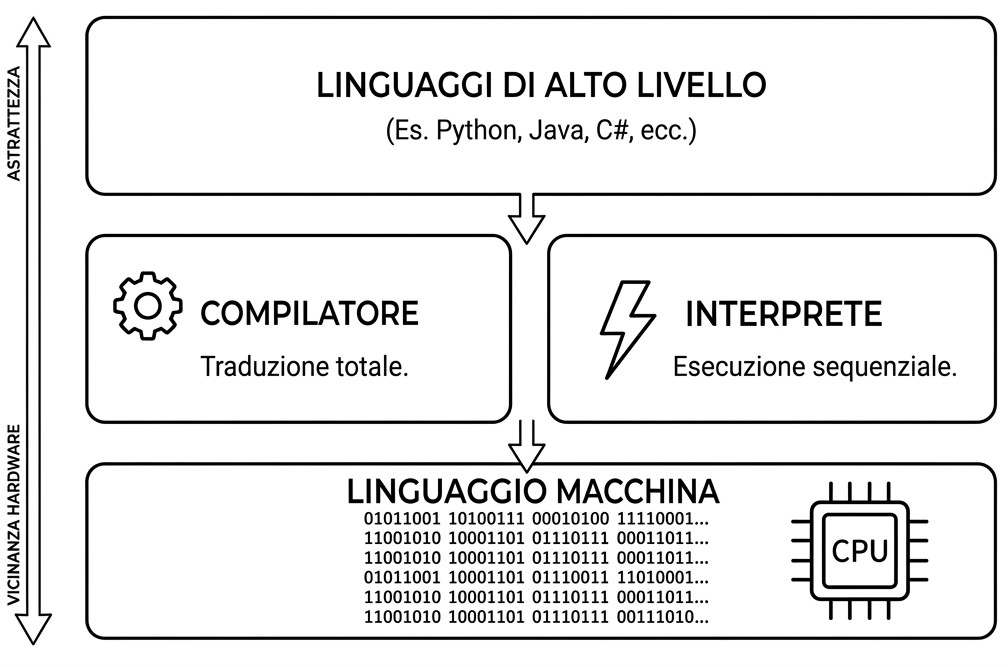
\includegraphics[width=\linewidth]{img/linguaggi.jpg}
                \caption{{creata con \href{https://gemini.google.com}{Gemini}}}
            \end{figure}
    \end{columns}
\end{frame}

\begin{frame}{Linguaggi di programmazione}
    \begin{alertblock}{CLASSIFICAZIONE DEI LINGUAGGI DI PROGRAMMAZIONE}
        \begin{minipage}{0.98\linewidth}
            \justifying
            Esistono diversi tipi di linguaggi di programmazione di alto livello, ciascuno 
            con un proprio \textbf{vocabolario} (inseme delle parole chiave) e una propria 
            \textbf{sintassi} (insieme delle regole da seguire per scrivere correttamente le istruzioni).\\ 
            Una classificazione dei linguaggi di programmazione può essere fatta in base al 
            \textbf{paradigma di programmazione}:      
            \begin{itemize}
                \pause
                \item \textbf{Programmazione imperativa}: Si concentra sulla descrizione passo dopo 
                passo di come viene eseguito un compito (es: C, Java, Python).
                \pause
                \item \textbf{Programmazione dichiarativa}: Si concentra sulla descrizione di ciò che si 
                desidera ottenere non sui passaggi per ottenerlo (es: SQL, Prolog).
                \pause
                \item \textbf{Programmazione orientata agli oggetti}: Si basa sulla concezione di un 
                programma come una collezione di oggetti che interagiscono tra loro (es: Java, C++, C\#, Python).
                \pause
                \item \textbf{Programmazione funzionale}: Si basa sul concetto di funzione matematica e 
                sulla composizione di funzioni pure (es: Scala).
            \end{itemize}
        \end{minipage}
    \end{alertblock}
\end{frame}

\section{PROPRIET\'A PYTHON}

\begin{frame}{PROPRIET\'A PYTHON}
    \begin{alertblock}{PROPRIET\'A PYTHON}
        \begin{minipage}{0.98\linewidth}
            \justifying
            \begin{itemize}
                \pause
                \item Python è un linguaggio \textbf{di alto livello}, \textbf{interpretato} e \textbf{multiparadigma};
                \pause
                \item Python è un linguaggio \textbf{non tipizzato}, ovvero non è necessario dichiarare il tipo di dato di una variabile prima di utilizzarla;
                \pause
                \item Python è un linguaggio \textbf{a tipizzazione dinamica}, ovvero il tipo di dato di una variabile può cambiare durante 
                l'esecuzione del programma;
                \pause
                \item Python è un linguaggio \textbf{case sensitive}, ovvero distingue tra maiuscole e minuscole.
                \pause
                \item Python è un linguaggio organizzato in \textbf{librerie importabili}, ovvero raccolte di 
                funzioni già pronte all'uso per svolgere compiti specifici.
                \bigskip
            \end{itemize}
        \end{minipage}
    \end{alertblock}
\end{frame}

\section{CONFIGURAZIONE AMBIENTE DI SVILUPPO}

\begin{frame}{AMBIENTE DI SVILUPPO}
    \begin{alertblock}{CONFIGURAZIONE}
        \begin{minipage}{0.98\linewidth}
            \justifying
            Per iniziare a programmare in Python è necessario configurare l' ambiente di sviluppo 
            installando i seguenti software:            
            \bigskip
            \begin{enumerate}
                \pause
                \item \textbf{\href{https://www.python.org}{Python}}: Python source code and installers; 
                \pause
                \item \textbf{\href{https://code.visualstudio.com/}{Visual Studio Code}}: IDE (Integrated development environment) editor per il codice sorgente;
                \pause
                \item \textbf{\href{https://marketplace.visualstudio.com/items?itemName=ms-python.python}{Estensione Python per VS Code}}: estensione per integrare Python in VS Code. 
            \end{enumerate}
            \bigskip   
        \end{minipage}
    \end{alertblock}
\end{frame}

\section{ESEMPIO CODICE PYTHON}

\begin{frame}{HELLOWORLD!}
    \begin{figure}
        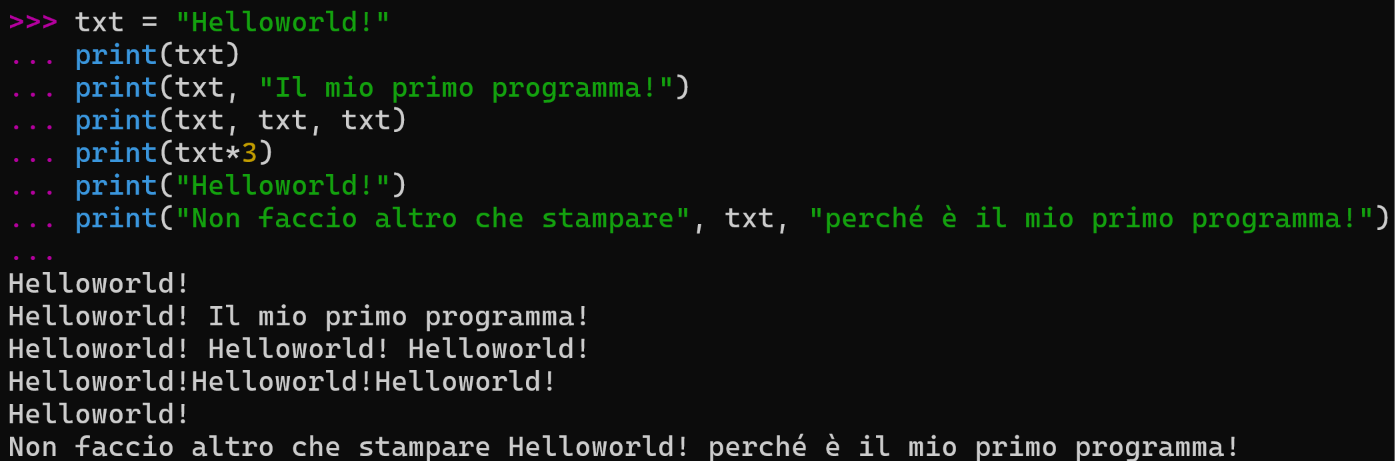
\includegraphics[width=\linewidth]{img/helloworld.png}
    \end{figure}
\end{frame}

\end{document}